

\textcite{han2011data}[363-365] list the following requirements  clustering methods must meet:
\begin{itemize}
  \item Scalability
  \item Ability to work with different attribute types
  \item Recognising clusters with arbitrary shapes
  \item Requirements for domain knowledge (for parameter selection)
  \item Ability to handle noise
  \item Incremental clustering (integrate updates without recomputation)
  \item Insensitivity to the order of the input
  \item Ability to cluster high-dimensional data 
  \item Capability to cluster under certain constraints
  \item Interpretability and usability of the results
\end{itemize}
% \begin{itemize}
%   \item Scalability: clustering algorithms need to work on large databases, which may contain millions or billions of entries.
%   \item Ability to work with different attribute types: The algorithm must be able to handle various data types, for example: binary, nominal (categorical), and ordinal data. More complex data types include graphs, sequences, images, and documents.
%   \item Recognising clusters with arbitrary shapes: Methods that use distance measures (e.g. Euclidean or Manhattan) to compute clusters usually find clusters of spherical shape. The size and density also tend to be similar. Clusters could however be of any shape, therefore the algorithms need to be capable of detecting any shape.
%   \item Requirements for domain knowledge: For some clustering algorithms, parameters (e.g. desired number of clusters) need to be determined. These can affect the cluster results. Parameters are hard to define, if the data is not understood.
%   \item Ability to handle noise (see section \ref{section:NoisyData})
%   \item Incremental clustering: The method should be able to integrate incremental data updates into existing structures, without recomputing the clustering.
%   \item Insensitivity to the order of the input: The clustering results should be the same, regardless of the order the objects are inserted into the algorithm.
%   \item Ability to cluster high-dimensional data (see section \ref{section:TheoryDimensionalityReduction}) %there is quite a good explanation here, but not really sure if need it
%   \item Capability to cluster under certain constraints %TODO: do i need an example constraint? not explained very well in the book
%   \item Interpretability and usability of the results
% \end{itemize}
% \begin{itemize}
%   \item Scalability: clustering algorithms need to work on large databases, which may contain millions or billions of entries.
%   \item Ability to work with different attribute types: The algorithm must be able to handle various data types, for example: binary, nominal (categorical), and ordinal data. More complex data types include graphs, sequences, images, and documents.
%   \item Recognising clusters with arbitrary shapes: Methods that use distance measures (e.g. Euclidean or Manhattan) to compute clusters usually find clusters of spherical shape. The size and density also tend to be similar. Clusters could however be of any shape, therefore the algorithms need to be capable of detecting any shape.
%   \item Requirements for domain knowledge: For some clustering algorithms, parameters (e.g. desired number of clusters) need to be determined. These can affect the cluster results. Parameters are hard to define, if the data is not understood.
%   \item Ability to handle noise (see section \ref{section:NoisyData})
%   \item Incremental clustering: The method should be able to integrate incremental data updates into existing structures, without recomputing the clustering.
%   \item Insensitivity to the order of the input: The clustering results should be the same, regardless of the order the objects are inserted into the algorithm.
%   \item Ability to cluster high-dimensional data (see section \ref{section:TheoryDimensionalityReduction}) %there is quite a good explanation here, but not really sure if need it
%   \item Capability to cluster under certain constraints %TODO: do i need an example constraint? not explained very well in the book
%   \item Interpretability and usability of the results
% \end{itemize}

% TODO: ON PAGE 356 - THERE ARE TECHNIQUES ON HOW TO COMPARE CLUSTERING METHODS - NOT SURE IF NEED

%TODO: check if all pages have been used - have been highlighting lines that have used test
%TODO IMPORTANT: this might not be 366-296 - depends on if i end up explaining in more detail - at end, find which pages i actually used


\textbf{todo: add images to compare how different methods cluster}


\textcite{han2011data}[366-368,373, 374, 385] present different clustering algorithms. They state, that it is not easy to divide these into distinct categories, since some algorithms share features from other categories. The general categories are partitioning methods, hierarchical methods, density-based methods and grid-based methods.

% (\textbf{Todo: Explain used methods in more detail after Experiment and add figures of graphs})
% \textbf{TODO: ONLY EXPLAIN IN DETAIL, WHICH METHODS ARE USED IN THE EXPERIMENT}
%TODO:maybe also look into performance comparisons
  \subsubsection{Partitioning Methods}
  Partitioning methods are the easiest and most significant types of clustering methods. The data is divided into \textit{k} (generally pre-defined) number of groups (clusters). The data consists of \textit{n} objects, thus \textit{k $\geq$ n}. Each group must contain at least one object. A data object can only be classified into one group (\textit{exclusive cluster separation}). Fuzzy partitioning methods relax this condition.
  Many of the partitioning methods use distance measures to calculate their clusters. If the number of clusters (\textit{k}) is pre-defined, then the clustering algorithm will create an initial segregation into \textit{k} clusters. Objects are then relocated to improve the partitioning. The partitioning is considered good, when objects assigned to the same cluster are "similar" and "dissimilar" from the objects in the other clusters. Traditional partitioning methods can also be applied onto subspaces (for many attributes and sparse data).  Examples: k-means, k-medoids \autocite{han2011data}[366, 368].
  




  \subsubsection{Hierarchical Methods}
  %CAREFUL!, sentence from book is similar:  A hierarchical clustering method works by grouping data objects into a hierarchy or “tree” of clusters.
  The data is grouped into a hierarchy ("tree") of clusters. Depending on how the hierarchical decomposition is constructed, there are two different approaches: \textit{agglomerative} or \textit{divisive}. In the \textit{agglomerative} or \textit{bottom-up} approach, each object creates its own cluster. Step by step it is then merged into its closest neighbours until all objects belong to one cluster, or a termination condition comes true. In the \textit{divisive} or \textit{top-down} approach, all objects initially form one cluster together. Step by step, each cluster is divided, until each object is contained in its own cluster, or a condition is met to terminate the process. Once a merge or split step has been performed, it cannot be reversed. Once merged/split, the objects also cannot swap cluster. Each merge or split decision influences the quality of the resulting clusters and must therefore be well chosen. Hierarchical methods can be used in subspaces and can use distance measures, or can be density- and continuity-based. Examples: BIRCH, Chameleon \autocite{han2011data}[366, 367, 373, 374].

  % todo COULD GO MORE INTO DETAIL ABOUT AGGLOMERATIVE AND DIVISIVE CLUSTERING, SEE PAGES 375-377 - but not sure if need, depends if being used

  
%TODO: PAPER BOOK PAGE 526 - quite interesting- linkage (how to determine distance between clusters)
  %TODO: CHECK, I THINK PARTITIONING AND HIERARCHICAL DON'T FILTER OUT NOISE AND OUTLIERS, BECAUSE THEY PARTITION THE ENTIRE DATA SET, SO EVERY OBJECT IS IN A CLUSTER. WOULD BE GOOD TO MENTION
  

  \subsubsection{Density-Based Methods}
  \label{section:densityBasedMethods}
  The majority of clustering methods (e.g. partitioning and hierarchical methods) use distance-based approaches, which results in only finding clusters with spherical shapes. Density-based methods have the ability to find clusters with random shapes. In these methods, objects are continuously added to the cluster, so long as the number of objects/data points (density) close by is larger than a given threshold. The clusters are comprised of high-density areas of objects. These are separated by spaces with low-density. Accordingly, this method is also useful for removing noise and outliers. These methods can also be used to cluster sub spaces. The following two density-based clustering algorithms were used in the experiment: DBSCAN and OPTICS.

  % Examples: DBSCAN, OPTICS, DENCLUE
  %TODO: page 385 - good figure of density based clustering - however might be better to fetch from a paper.



\paragraph{DBSCAN}
\label{section:DBSCAN}
\textcite{DBSCAN}[226-229] introduce a new density-based clustering algorithm, the Density Based Spatial Clustering of Applications with Noise. This method is able to find clusters with different shapes and work efficiently on large spatial datasets. The algorithm searches in a given radius (Eps = epsilon parameter) around a data point. If within this radius a minimum number of points (MinPts parameter) exists, then this point is added to the cluster (core point). A data point (\textit{p}) is considered a border point, if inside of its Eps neighbourhood there is a core point (\textit{q}). A data point is labelled as noise, if it does not belong to any clusters (has no core points within the given radius).
% The goal is to keep adding neighbouring data points to the cluster
% In doing so, core points and border points are distinguished.
%todo: rewrite - that uses two global parameters instead of one - or say that only with one paramter
According to \textcite{han2011data}[388], a weakness of DBSCAN is the fact that the results rely on the chosen parameters. If these are selected differently, the clustering results can differ. These parameters can often be challenging to select.

\textcite{DBSCAN}[230] supports the selection of the Eps and MinPts parameters. The idea is to select the appropriate parameters for the "thinnest" cluster. The first step is to construct a sorted k-dist graph. For a specific \textit{k}, calculate the distance \textit{d} of every point \textit{p} to its \textit{k}th nearest neighbour. Sort these distances in descending order and depict them on a graph. Such a graph can be seen in figure \ref{figure:sortedKGraphDBSCAN}. The goal is to locate the \textit{threshold} of the highest distance to the \textit{k}th nearest neighbour (the "thinnest" cluster). The first point in the "valley", as can be seen at the tip of the arrow in figure \ref{figure:sortedKGraphDBSCAN}, is this threshold point. The points to the left with higher distances are likely to be noise and the points to the right are part of clusters. The authors suggest selecting 4 for \textit{k}. Experiments have shown that the results for higher values for \textit{k} do not vary greatly. They therefore recommend defining MinPts as 4 and using a 4-dist graph to estimate the Eps parameter.


\begin{figure*}[h]
  \centering
  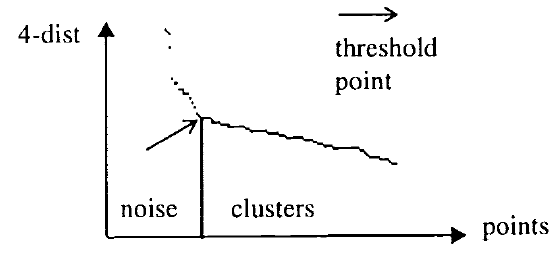
\includegraphics[width=0.5\textwidth]{./images/sortedKGraphDBSCAN.png}
  \caption{Sorted 4-dist graph (distance for each point to its fourth nearest neighbour) \autocite{DBSCAN}[230].}
  \label{figure:sortedKGraphDBSCAN}
\end{figure*}

% d = distance of point p to its k-th nearest neighbourhood
% d-neighbourhood of p contains more than k+1 points - if several points have the same distance d from p as the kth point - unlikely
%map each point from database to the distance from its kth nearest neighbour - sort in descending order - graph gives hints concerning density distribution in the db (= sorted k-dist graph)



\paragraph{OPTICS}
\label{section:OPTICS}
\textcite{han2011data}[388] mention, that OPTICS was created to improve the selection of global parameters problem in DBSCAN.
\textcite{OPTICS}[49, 51-54, 57, 60] present the density base clustering algorithm OPTICS (Ordering Points To Identify the Clustering Structure). This method in itself does not specifically create clusters. Instead, it orders the dataset according to its density-based clustering structure. For each object, the values \textit{core-distance} and \textit{reachability-distance} are calculated. The \textit{core-distance} of an arbitrary data point (object) \textit{o} is the distance to the nearest point within Eps that completes the MinPts rule and therefore labels point \textit{o} as a core point. If there is not the number of MinPts in the Eps neighbourhood, then the \textit{core-distance} of that point is undefined. The \textit{reachability-distance} of an object \textit{p} to core object \textit{o} is defined as the max value of the core-distance and the distance from object \textit{o} to object \textit{p}. Likewise, if \textit{o} is not a core object, then the \textit{reachability-distance} of \textit{p} is undefined. The \textit{core-distance} and \textit{reachability-distance} are visualised in figure \ref{figure:reachabilityDistanceOPTICS}.

\begin{figure*}[h]
  \centering
  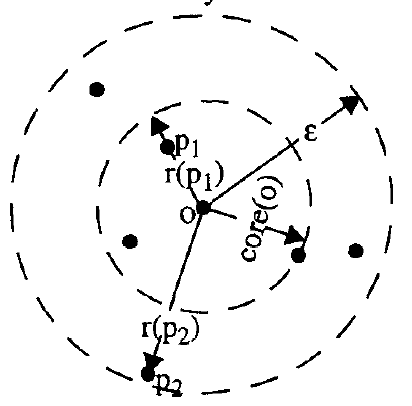
\includegraphics[width=0.3\textwidth]{./images/reachabilityDistanceOPTICS.png}
  \caption{Core-distance of object \textit{o} (MinPts = 4) and reachability-distances for objects \textit{p1} and \textit{p2} \autocite{OPTICS}[52].}
  \label{figure:reachabilityDistanceOPTICS}
\end{figure*}
%TODO: i wrote this from the paper - not sure whether to add - end is missing - see optics page 53 - pseudo code explanation
%The OPTICS algorithm takes an arbitrary core point, and orders its directly density-reachable objects (according to Eps and MinPts) and sorts them by their reachability-distance (to the selected core point). From the smallest to the largest reachability-distance, each point is selected and added to an OrderedFile, along with its calculated core-distance and reachability-distance.

The data points are ordered by the OPTICS algorithm (using their reachability-distance) to create a reachability plot. This plot is relatively stable towards the input parameters. In figure \ref{figure:reachabilityPlotOPTICS} a reachability plot calculated from a 2D dataset is depicted. 

\begin{figure*}[h]
  \centering
  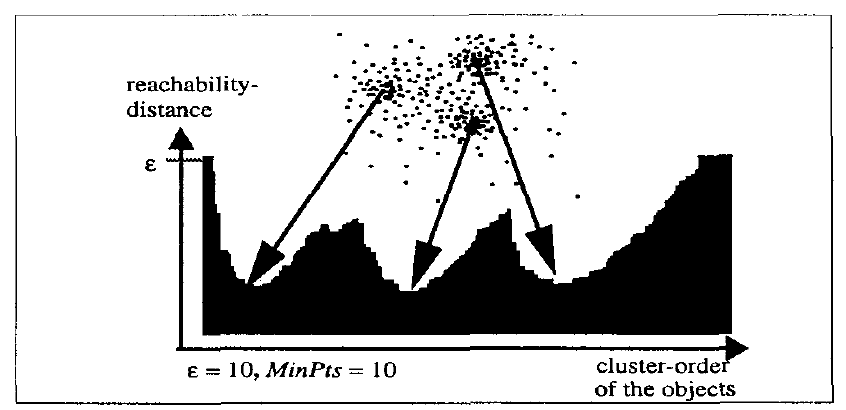
\includegraphics[width=0.5\textwidth]{./images/reachabilityPlotOPTICS.png}
  \caption{OPTICS reachability plot for a 2D dataset. Three "Gaussian bumps" can be seen \autocite{OPTICS}[54].}
  \label{figure:reachabilityPlotOPTICS}
\end{figure*}

The clusters can then be automatically constructed from the reachability plot by pinpointing the start-of-cluster and end-of-cluster regions and combining regions that match into clusters (or nested clusters). Since the reachability-distance of a point is the distance from the set of its predecessors and through OPTICS' specific ordering, the clusters are the dips in the reachability plots (as can also be seen in figure \ref{figure:reachabilityPlotOPTICS}). In figure \ref{figure:clusterExtractionOPTICS}, a cluster could hence be extracted from this plot starting at the 3rd data point and ending with the 16th.


\begin{figure}
  \centering
  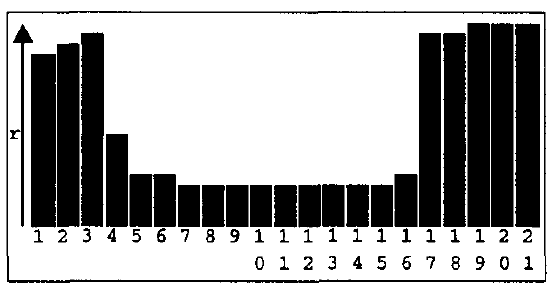
\includegraphics[width=0.5\textwidth]{./images/clusterExtractionOPTICS.png}
  \caption{Since clusters are defined as the dips/dents in the reachability plots created by the OPTICS algorithm, a cluster can be extracted from this plot starting at the 3rd data point and ending with the 16th. The x-axis of the reachability plot depicts the order of the data points (objects) and the y-axis the reachability-distance for each datapoint \autocite{OPTICS}[57].}
  \label{figure:clusterExtractionOPTICS}
\end{figure}

%todo: In comparison to DBSCAN - problem with containment - optics page 52

 

  \subsubsection{Grid-Based Methods}
  %not sure if correct - sentence from book page 367: The main advantage of this approach is its fast processing time, which is typically independent of the number of data objects and dependent only on the number of cells in each dimension in the quantized space.
  The previously mentioned clustering methods are data-driven (they accommodate the distribution of the data objects). Grid-based methods are space-driven (they do not rely on the distribution of the data objects). The data objects are quantised into grid cells on a multiresolution grid. The actions required for clustering are performed on the grid structure. The processing time depends on the grid size (number of cells) in each dimension and not on the number of objects and is more accelerated than other clustering methods. Examples: STING, CLIQUE \autocite{han2011data}[367, 392].
  
  

  \vspace{5mm} %5mm vertical space
\textcite{han2011data}[414, 416] clarify, that the clustering methods mentioned above have a good functionality when used on a dataset with fewer than 10 attributes. Another way to cluster high-dimensional data is \textit{subspace clustering}, in which subspaces (subset of attributes) are investigated to find clusters. The CLIQUE method is used for subspace clustering. 


  %TODO: paper book page 542 - kohonen networks